\question{Электроразрядные способы накачки в газовых лазерах}

Газовый лазер накачивается электрическим разрядом при пропускании через 
газовую смесь тока -- постоянного, радиочастотного (СВЧ) или импульсного. 
Обычно ток протекает через газовую среду либо вдоль оси лазера 
(продольный разряд, рис.~\ref{img22.1}а), либо перпендикулярно ей (поперечный 
разряд, рис~\ref{img22.1}б). Поскольку поперечные размеры активной среды 
обычно гораздо меньше её продольных размеров, то для одной и той же газовой 
смеси требуемое напряжение при поперечной конфигурации накачки существенно 
меньше, чем при продольной. С другой стороны, продольный разряд, ограниченный 
диэлектрической трубкой зачастую является более пространственно однородным и 
устойчивым источником накачки. 

Для стабилизации тока разряда в требуемой рабочей точке необходимо 
использовать последовательное сопротивление \( R_B \), часто называемое 
балластным сопротивлением. 

\begin{figure}[h!]
    \center
    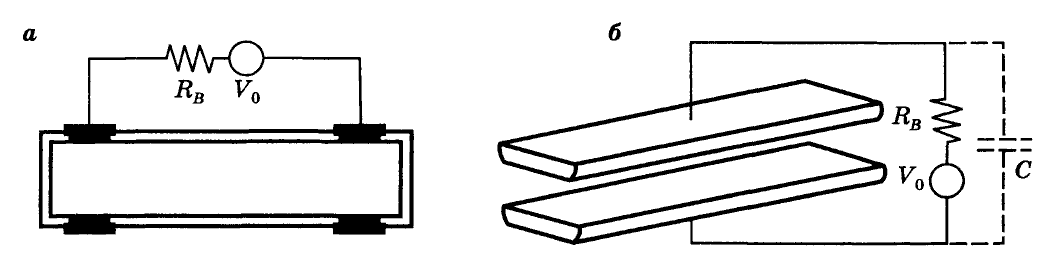
\includegraphics[width=.4\textwidth]{22_01}
    \caption{Наиболее часто используемые конфигурации накачки в газовых 
    	лазерах: (а) продольный разряд и (б) поперечный разряд}
    \label{img22.1}
\end{figure}

При электрическом разряде образуются как ионы, так и свободные электроны. 
Поскольку эти заряженные частицы получают в приложенном электрическом поле 
дополнительную кинетическую энергию, то в результате столкновения с 
нейтральной частицей они способны возбудить её. Положительные ионы из-за 
своей значительно большой массы ускоряются до гораздо меньших скоростей, чем 
электроны, и в связи с этим не играют заметной роли в процессах возбуждения. 
Таким образом, электрическая накачка газовой среды обычно происходит в 
результате одного или обоих из следующих двух процессов:
\begin{enumerate}
	\item в газе, состоящем из частиц одного вида, возбуждение осуществляется 
		только электронным ударом, то есть в процессе 
		\[ e = X \rightarrow X^{*} + e \]
		где через \( X \) и \( X^{*} \) обозначена частица соответственно в 
		основном и возбужденном состояниях. Такой процесс называют 
		столкновение первого рода;
	\item в газе, состоящем из частиц двух видов (назовём их \( A \) и 
		\( B \)), возбуждение может происходить также при столкновении двух 
		частиц разных видов посредством резонансной передачи энергии.
\end{enumerate}

\begin{figure}[h!]
    \center
    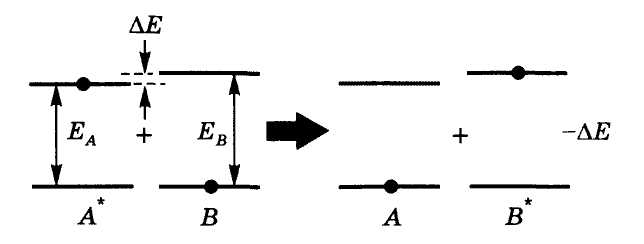
\includegraphics[width=.4\textwidth]{22_02}
    \caption{Лазерная накачка при квазирезонансной передаче энергии}
    \label{img22.2}
\end{figure}

Обратившись к рис.~\ref{img22.2}, предположим, что частица \( B \) находится в 
основном состоянии, а частица \( A \) возбуждена электронным ударом. Предположим 
также, что абсолютная величина разности энергий \( \D E \) возбужденных 
состояний этих частиц меньше, чем \( kT \). В этом случае существует 
значительная вероятность того, что после их столкновения частица \( А \) 
окажется в основном, а частица \( В \) -- в возбужденном состоянии. Этот 
процесс можно представить в виде
\[
	A^{*} + B \rightarrow A + B^{*} - \D E
\]
где разность энергий \( \D E \), в зависимости от своего знака, добавляется к 
кинетической энергии сталкивающихся частиц или вычитается из нее; вот почему 
по абсолютной величине \( \D E \) должна быть меньше, чем \( kT \). Указанный
процесс оказывается особенно эффективным способом возбуждения частиц \( B \), 
если верхнее состояние частиц \( A \) является метастабильным (т. е. 
излучательный переход из него запрещен). В этом случае после того, как частица 
\( A \) переведена в возбужденное состояние, она будет оставаться в нем в 
течение длительного времени, являясь энергетическим резервуаром для 
возбуждения частиц \( B \). Процесс такого типа называют столкновением второго 
рода.
